\documentclass{article}
\usepackage{lmodern}
\usepackage[main,preprint]{neurips_2026}
\usepackage[utf8]{inputenc}
\usepackage[T1]{fontenc}
\usepackage{amsmath,amssymb}
\usepackage{graphicx}
\usepackage{booktabs}
\usepackage{microtype}
\usepackage{xcolor}
\usepackage{url}
\usepackage{hyperref}
% Caption macros for all delivered assets. Requires amsmath for mathematics.
\newcommand{\BudgetCurvesCaption}{Minimum task budgets under full gains. Each curve is the fraction of a common challenger cohort that can attain co-first by changing at most $k$ tasks to score one, holding rivals' task scores fixed and recomputing Borda ranks. Challengers exclude the union of all five rules' incumbent winners in this setting: 77 of 79 HELM MMLU evaluations (v1.13.0), and 4,571 of 4,575 Open LLM evaluations (normalized scores; snapshot \texttt{9c09a7cae433}). Curves use exact or certified optimal counts; all targets are reachable. Rules weight tasks equally; ties within $10^{-10}$ count as co-first. The horizontal guide marks 50\%. These are finite-cohort descriptions, with no sampling confidence bands. A task count measures a hypothetical score intervention, not training resources; task units differ between benchmarks.}
\newcommand{\GainReachabilityCaption}{Reachability depends on the gain constraint. A selected task changes from $x_j$ to $x_j+\alpha(1-x_j)$; rivals' task scores remain fixed, and Borda ranks are recomputed. Points show the fraction reaching co-first with any allowed task budget, on fixed full cohorts of 79 HELM and 4,575 Open LLM evaluations, including incumbent winners. Infeasible targets remain in the denominator. Connecting lines guide the eye between the four evaluated gain settings, not a fitted dose--response. At $\alpha=0.25$, all Open LLM evaluations are reachable under minimum, while most are unreachable under the other rules. Scores, snapshots and tie conventions match Figure~\ref{fig:budget}. No causal training effect or sampling uncertainty is estimated.}
\newcommand{\TaskCompositionCaption}{Sensitivity to task composition under full gains and unit ceilings. Each value is a design's median minimum task budget, using all 79 HELM or 4,575 Open LLM evaluations, including incumbents. Left: 200 seeded resamples of 57 HELM subjects with replacement; thin segments show the full observed range, thick segments the central 95\% empirical range, and open circles the median across designs. Right: six designs each delete one Open LLM task, leaving five tasks; dot area is proportional to the number of designs at a value, and segments join their observed extrema. These are composition sensitivities, not confidence intervals for published task scores. Cohorts differ from the primary challenger figures.}
\newcommand{\CohortsCaption}{Frozen public score matrices and primary target cohorts. HELM uses subject-level exact-match scores; Open LLM uses published normalized task scores divided by 100. Challenger cohorts remove the union of all five incumbent-winner sets under full gains and unit ceilings. Open LLM retains evaluations at different precisions separately; one-evaluation-per-model filtering is a sensitivity. Full source hashes and exclusion audits accompany the code.}
\newcommand{\PrimaryBudgetsCaption}{Median minimum selected-task budgets, with task fractions, on the common primary challenger cohorts (HELM: 77 evaluations and 57 tasks; Open LLM: 4,571 evaluations and six tasks). All targets are reachable under full gains to score one. Co-first permits ties within $10^{-10}$. Values are descriptive finite-cohort medians, not measured training costs or estimates with score-level confidence intervals.}
\newcommand{\PairedBordaCaption}{Exact paired comparisons under full gains and unit ceilings. Each target is compared with itself under Borda and the named rule, using the common challenger cohort; all paired targets are reachable. Entries count targets for which Borda needs fewer, equal, or more selected tasks. Borda is never cheaper than mean or geometric on these particular cohorts, but is cheaper than minimum for some targets in both snapshots, and cheaper than median for some Open LLM targets. This supports no universal ordering across arbitrary score matrices.}
\newcommand{\RobustnessCaption}{Sensitivity of median minimum task counts under full gains to score one. HELM range and central 95\% columns summarize 200 task-resampling designs; Open deletions gives the range over six five-task designs. These columns use all evaluations, including incumbents, and represent composition sensitivity, not test-score confidence intervals. Open raw uses raw rather than published normalized scores on 4,575 evaluations; Open unique uses a deterministic one-evaluation-per-model cohort of 4,496. Those columns use six tasks and their own full cohorts, and should not be pooled with the primary challengers.}
\newcommand{\RandomSelectionCaption}{Targeted versus uniformly random task selection, using all 79 HELM or 4,575 Open LLM evaluations, including incumbent winners. Each entry is a cohort mean of the minimum optimal count or the first-success count for a random task order, under full gains and unit ceilings. All targets are reachable, so the analysis's $n+1$ censoring code is unused. HELM random means use 256 independent seeded permutations per target; the interval column gives conservative 95\% Hoeffding intervals for Monte Carlo error of the cohort mean. Open LLM random expectations are exact over subsets, with no Monte Carlo error. Intervals do not measure uncertainty of published model scores.}
\newcommand{\CeilingSensitivityCaption}{Median minimum task counts with a unit ceiling versus each task's best observed score as its ceiling. Gains are full ($\alpha=1$); the primary common challenger cohorts are unchanged (77 HELM, 4,571 Open LLM), and all targets remain reachable. Costs count selected tasks, and co-first permits ties within $10^{-10}$. The best-observed ceiling is a score constraint, not evidence that targeted training can attain it.}

\title{How many tasks buy first place?\\Exact score-space budgets for multi-task leaderboards}
\author{ResearchWorld study}
\begin{document}
\maketitle
\begin{abstract}
How much targeted improvement is needed to put a model first on a multi-task leaderboard? We define investment as the minimum number of task scores raised under an explicit improvement menu, holding rivals' underlying scores fixed. This measures intervention breadth in score space; it does not estimate training data, compute or achievable training gains. We give exact solutions for arithmetic mean, median, geometric mean, minimum and Borda aggregation, including the effect of target improvements on rivals' Borda totals. On frozen HELM MMLU and Open LLM Leaderboard score matrices, primary common challengers require median budgets of 16 versus 48 of 57 subjects, and 2 versus 6 of 6 tasks, for mean versus Borda when selected scores reach the unit ceiling. Borda is never cheaper than mean on those primary challenger cohorts, but there is no universal ordering across rules or assumptions. At quarter-headroom gains, most targets become infeasible under several rules, while every Open LLM target remains reachable under minimum aggregation. Normalization and task composition further qualify the comparison. Public snapshots, subset witnesses, optimizer validation, random-selection baselines and sensitivity analyses make these conditional conclusions reproducible.
\end{abstract}
\section{Introduction}
A multi-task leaderboard compresses a vector of task scores into a ranking. That compression determines not only which model looks strongest, but also which improvements most efficiently change the winner. If a developer can focus effort on selected evaluation tasks, how many tasks must improve before a specified model reaches first place, and how does that number depend on the aggregation rule?

This question requires an explicit intervention model. The number of training examples, training compute and attainable score gains are not observed in public score tables. We therefore study a conditional, directly checkable quantity: the smallest number of task coordinates that must be raised, according to a stated gain law, for a target to become co-first. A unit of investment is access to one task's prescribed score improvement. This isolates the interaction between aggregation and selective improvement. It cannot identify the cost or effectiveness of an actual training procedure.

We compare arithmetic mean, conventional median, geometric mean, minimum and Borda aggregation on two frozen public leaderboards. Our main intervention sets selected scores to the unit ceiling, an intentionally generous upper envelope of score access. We then restrict improvements to fractions of the available headroom, replace the ceiling by observed task maxima, require strict first place, and perturb score representation, rival cohorts and task composition. Rivals' underlying scores remain fixed, but their Borda totals are recomputed when the target passes them.

The primary common-challenger medians for mean versus Borda are 16 versus 48 of 57 HELM subjects and 2 versus 6 of 6 Open LLM tasks. Borda is never cheaper than mean on these primary cohorts. Yet bounded gains strongly change reachability, normalization changes minimum aggregation materially, and individual targets violate other rule orderings. Our contribution is an auditable conditional comparison: exact per-target budgets, shared-cohort rule comparisons and sensitivity evidence identifying where conclusions change. Related work already establishes voting-based evaluation and several strategic mechanisms; we make no priority claim about the general question.

\section{Related work}
MMLU supplies diverse subject-level assessments \citep{hendrycks2021mmlu}; HELM situates accuracy within a broader collection of scenarios and metrics \citep{liang2023helm}. BBH illustrates that a benchmark family can itself aggregate heterogeneous tasks \citep{suzgun2022bbh}. Our equal-subject MMLU design and six-column Open LLM design analyze particular task units, rather than reproducing every published leaderboard weighting or evaluating all dimensions of model quality. The Benchmark Lottery shows how benchmark choices affect method comparisons \citep{dehghani2021lottery}, motivating our composition checks.

\citet{lanctot2023socialchoice} already treat tasks as voters and agents as alternatives and study voting methods for evaluation, including Borda. Our comparison uses one ordinal rule alongside four cardinal summaries; it does not survey social-choice methods or test their recommendations for maximal lotteries. Constructive voting bribery asks whether constrained edits can make a preferred candidate win \citep{faliszewski2016bribery}. Target-only upward rank changes offer a useful analogy, but our restricted score-ceiling menu has its own optimization structure; no general bribery-complexity claim is imported.

Contamination studies demonstrate that benchmark-related training information can inflate scores and that cross-task effects matter \citep{zhou2023cheater,yang2023rephrased}. They motivate selective improvement without calibrating our gain menu to a training dose. Selective disclosure and uneven data access in Arena are distinct strategic mechanisms \citep{singh2025illusion}. A designer--developer game with endogenous strategic post-training \citep{chen2026incentives} studies interactions among developers and the benchmark designer. We instead hold rival score rows fixed and ask an exact reachability question for one target. We claim a reproducible conditional comparison of intervention breadth, not the introduction of voting-based evaluation, a prediction of strategic equilibria, evidence that listed models are contaminated, or priority for the general research question.

\section{Investment as a score intervention}
\label{sec:methods}
Let $X\in[0,1]^{m\times n}$ contain higher-is-better scores for $m$ evaluations on $n$ tasks. For target $t$, choose $S\subseteq\{1,\ldots,n\}$ and define
\begin{equation}
 x'_{tj}=x_{tj}+\mathbb{1}\{j\in S\}\alpha(u_j-x_{tj}),
 \label{eq:intervention}
\end{equation}
where $\alpha\in(0,1]$ and $u_j\geq\max_i x_{ij}$. All other rows remain fixed. We measure investment as $|S|$, also reporting $|S|/n$ within each benchmark. Equal task costs make a transparent combinatorial budget; subjects with different sizes and difficulties need not have equal training costs. Independent task improvements, no adverse cross-task effects, complete knowledge of the matrix and unconstrained subset selection are assumptions.

For aggregation rule $A$, let $A_i(X)$ be evaluation $i$'s aggregate. The minimum co-first budget is
\begin{equation}
 K_A(t;\alpha,u)=\min_S\{|S|: A_t(X')\geq\max_{i\ne t}A_i(X')\},
 \label{eq:budget}
\end{equation}
with $K_A=\infty$ if no subset succeeds. Existing winners have $K_A=0$. Co-first permits a numerical tolerance of $10^{-10}$; strict-first is analyzed separately. The main setting is $\alpha=1,u_j=1$. Sensitivities use $\alpha\in\{0.5,0.25,0.1\}$ at unit ceiling, and $\alpha=1,u_j=\max_i x_{ij}$. The observed-maximum ceiling limits gains to scores already represented in the snapshot; it still assumes the target can attain them.

\paragraph{Rules.}
We select four cardinal summaries to cover additive gains, central performance, multiplicative balance and weakest-task performance, plus one ordinal rule based on task ranks. This is a controlled recomputation of alternative rules on the same matrix, not a claim that each is deployed by the source leaderboard. We weight tasks equally. The mean is $n^{-1}\sum_j x_{ij}$; the geometric mean is $(\prod_j x_{ij})^{1/n}$, retaining zeros; the minimum is $\min_j x_{ij}$. The median is the central order statistic for odd $n$, or the average of the two central values for even $n$. For Borda, define $p(a,b)=\mathbb{1}\{a>b\}+\tfrac12\mathbb{1}\{a=b\}$ and
\begin{equation}
 B_i(X)=\sum_j\sum_{\ell\ne i}p(x_{ij},x_{\ell j}).
\end{equation}
This is the sum of average ascending task ranks minus one; higher is better. Its units differ from the cardinal scores, but $K_A$ has the same task-count units for every rule. The strongest rival can differ by rule, an essential part of the comparison.

\paragraph{Exact cardinal solutions.}
For a cardinal rule, rivals' aggregates remain fixed. Let $H$ denote the largest rival aggregate and $y_j=x_{tj}+\alpha(u_j-x_{tj})$ the allowed improved score. For the mean, select the shortest prefix of descending gains $y_j-x_{tj}$ whose sum reaches $nH-\sum_j x_{tj}$. Exchanging a selected smaller gain for an unselected larger one cannot hurt, proving optimality for unit costs. For a positive geometric threshold, first force upgrades of all zero coordinates; an unremovable zero implies infeasibility. Sort the remaining log gains and apply the same argument.

For $n=2h-1$, median success requires at least $h$ coordinates at least $H$. If $q$ already meet $H$, select $\max(0,h-q)$ eligible coordinates that can reach it; insufficient eligible coordinates imply infeasibility. Thus full unit-ceiling improvement requires at most $h$ selections. This argument does not apply to the conventional even median: all subsets are enumerated for the six-task benchmark. For the minimum, every coordinate below $H$ must reach $H$; their count is exact if all are eligible, and otherwise the target is infeasible. A low rival minimum can make this requirement inexpensive even when the target trails on many other metrics.

\paragraph{Borda with moving rival totals.}
Let $d_{ij}=p(y_j,x_{ij})-p(x_{tj},x_{ij})$ for $i\ne t$ and $g_j=\sum_{i\ne t}d_{ij}$. Selecting $j$ gains $g_j$ target points and removes $d_{ij}$ rival points. With binary $z_j$ the exact optimization is
\begin{align}
 \min_z\;&\sum_j z_j \quad \text{subject to}\nonumber\\
 &\sum_j(g_j+d_{ij})z_j\geq B_i(X)-B_t(X),\quad i\ne t.
 \label{eq:borda}
\end{align}
Freezing rivals' Borda totals would solve a different problem. We solve this binary program with zero relative optimality gap for HELM, and enumerate all subsets for Open LLM. Strict Borda first place raises the required gap by half a point, since scores are half-integral. Cardinal strict-first uses the stated numerical tolerance. Each feasible subset is checked directly against the winning condition.

For all five rules, improving target coordinates cannot worsen its relative position. Accordingly $K_A$ is nonincreasing in $\alpha$ and in the ceiling, treating infeasibility as infinity. This supplies a diagnostic, not an ordering between rules. Heterogeneous task costs would invalidate the sorted-gain count argument; coupled gains or changing rivals would change the feasible intervention set itself.

\section{Data and experimental design}
\label{sec:design}
\paragraph{Frozen public matrices.}
HELM MMLU~\citep{hendrycks2021mmlu,liang2023helm} release v1.13.0 (dated 2025-01-10) supplies exact-match scores for 79 models on all 57 MMLU subjects. All rows are complete; no model is removed for missing scores. The source's evaluation counts range from 100 to 1,534 across reported cells. Equal subject weighting therefore differs from pooling all test examples and is a study design, not an assertion that we reproduce HELM's displayed aggregate weighting. Open LLM Leaderboard contents~\citep{openllmcontents2025} at commit \texttt{9c09a7cae43334062a82cb164f2ef255013dafa2} supplies 4,576 evaluations on IFEval, BBH, MATH Level 5, GPQA, MUSR and MMLU-PRO. We exclude one source-flagged evaluation and retain 4,575 complete rows. Primary scores are the six published normalized columns divided by 100; we verify their mean exactly reproduces the published average. These matrices are analyzed separately: a subject and a broad task are different units of investment.

Open LLM rows identify model--precision evaluations, so related models and repeated model names are not independent experimental draws. We retain the public evaluation population for the primary comparison and use a deterministic one-row-per-model-name sensitivity with 4,496 entries. A separate sensitivity uses the six raw score columns in their supplied $[0,1]$ units. HELM has no zero cells; the primary Open LLM matrix has 384. We preserve zeros rather than adding offsets to geometric means. Acquisition on 2026-11-03 records all URLs, byte counts and SHA-256 hashes in \texttt{data/manifest.json}; preparation and exclusion counts are in \texttt{data/processed/audit.json}.

\paragraph{Cohorts and outcomes.}
We compute budgets for every retained target, all five rules and all five gain/ceiling settings. For primary paired comparisons we remove the \emph{union} of incumbent winners across rules, leaving 77 HELM and 4,571 Open LLM common challengers. This avoids comparing a zero-cost incumbent for one rule with a genuine challenger for another. We also report the full cohorts, with incumbents included. Bounded-gain reachability uses those fixed full cohorts; conditioning budgets on rule-specific reachable subsets would confound the comparison with a change in targets. We report budget distributions, paired counts and the fraction reachable within each budget. Infeasible targets stay in the denominator.

\paragraph{Random task selection.}
A baseline selects tasks in a uniformly random order and applies the same intervention until co-first. On six tasks, success at each budget is the exact fraction of subsets of that size which succeed. The expected first-success count follows from the survival probabilities. For HELM we use 256 independent random task permutations per reachable target and setting, seed 20261103. If no subset can succeed, a stopping code of $n+1$ denotes censoring, not an achievable investment. Full-cohort censored stopping means assign that known value to every provably infeasible target; success probability at a target's own optimal budget is defined only when that budget is finite and is labelled reachable-only with its denominator. Main full-gain comparisons have no infeasible targets. Wilson intervals describe per-target Monte Carlo success probabilities; conservative Hoeffding intervals describe cohort-mean stopping counts. Neither estimates uncertainty in the published model scores.

\paragraph{Sensitivity and verification.}
We repeat the full intervention grid for strict first place; analyze raw scores and unique model names at the primary setting; resample 57 HELM task columns with replacement in 200 seeded designs; and delete each of the six Open LLM tasks in turn. These perturbations assess dependence on benchmark composition. They are not confidence intervals for latent model quality. Scores are fixed published aggregates without repeated runs sufficient to estimate evaluation noise. All 278,055 attack records finish with exact/optimal or infeasible status and zero unresolved optima. We additionally check monotonicity, independently recompute 400 reported winners including full Borda reranking, and compare optimizers against exhaustive enumeration in 120 small validation cases with ties and zeros (seed 47). These validation cases check algorithms and are excluded from empirical claims.

\section{Results}
\label{sec:results}
\subsection{Full improvements separate Borda from cardinal rules}
Table~\ref{tab:primary} and Figure~\ref{fig:budget} report the common-challenger comparison. Under full unit-ceiling improvement, every target can reach co-first for every rule. On common challengers, median budgets for mean, median, geometric mean, minimum and Borda are respectively 16, 21, 16, 12 and 48 of 57 HELM subjects; Open LLM medians are 2, 3, 3, 3 and 6 of 6 tasks. These are finite-cohort descriptions of optimal task counts. They are neither estimates of training resources nor comparisons of equal effort between benchmarks.

\begin{table}[t]
\caption{\PrimaryBudgetsCaption}
\label{tab:primary}
\centering
\input{tables/primary_budgets}
\end{table}
\begin{figure}[t]
\centering
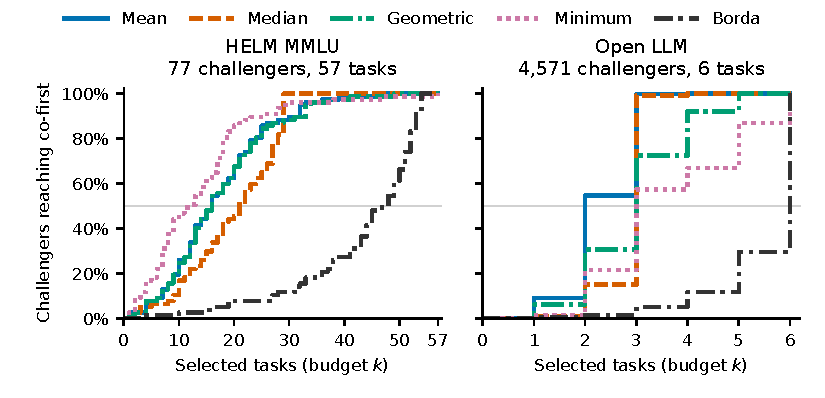
\includegraphics[width=\linewidth]{figures/budget_curves.pdf}
\caption{\BudgetCurvesCaption}
\label{fig:budget}
\end{figure}

The paired comparison (Appendix Table~\ref{tab:paired}) is stronger than a comparison of medians alone. Every HELM common challenger needs more selections under Borda than mean. For Open LLM, Borda costs more for 4,544 challengers and ties for 27; none is cheaper. The same zero-cheaper result holds against geometric mean in these primary cohorts. Yet this is not a universal ordering of the five rules: Borda is cheaper than minimum for one HELM challenger and 16 Open LLM challengers, and cheaper than median for 16 Open LLM challengers. Mean is cheaper than median for 64 HELM challengers, ties for two, and costs more for 11. The full per-target records and paired counts allow these exceptions to be checked.

Including incumbents changes the HELM Borda median from 48 to 46 and minimum from 12 to 11; other HELM medians and all Open LLM medians above are unchanged. The lone full-cohort Open LLM case in which Borda is cheaper than mean is Borda's existing winner, whose budgets are zero and one. Removing the common incumbent union prevents this special case from being mistaken for a challenger advantage.

The mechanism is consistent with the exact formulations. Mean improvements can concentrate on large score gaps; median success depends on crossing a threshold in enough coordinates; minimum success depends on repairing every coordinate below a possibly low rival minimum. Borda converts each task improvement into rank crossings against all rivals. Reaching the cardinal ceiling can therefore buy many cardinal-score units without buying sufficient rank points to overtake a broad-task leader. The empirical separation arises from these observed profiles and opponents, rather than from a theorem that Borda always requires more tasks.

\subsection{Restricting gains changes who can reach first}
Figure~\ref{fig:gain} shows fixed-cohort reachability. At quarter-headroom improvement ($\alpha=0.25$, unit ceilings), reachable HELM counts for mean, median, geometric mean, minimum and Borda are 9, 11, 9, 21 and 10 out of 79. Open LLM counts are 558, 427, 841, 4,575 and 480 out of 4,575. The minimum remains reachable for every Open LLM target while most targets are infeasible under the other rules. Its first-place threshold is the largest rival's weakest score; it need not require uniformly high scores. Thus a rule that penalizes weak tasks can still permit inexpensive selective improvements relative to its own leader.

\begin{figure}[t]
\centering
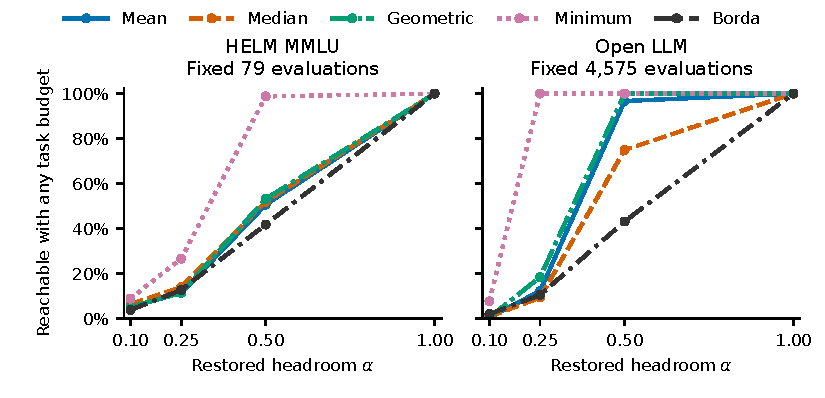
\includegraphics[width=\linewidth]{figures/gain_reachability.pdf}
\caption{\GainReachabilityCaption}
\label{fig:gain}
\end{figure}

The fixed-cohort reachability curves show this change without silently removing hard targets. Smaller medians among reachable targets would not demonstrate increased robustness or vulnerability: a tighter gain constraint changes the reachable cohort. The observed-maximum ceiling offers a second intervention restriction using scores already achieved in the snapshot; its full results are included with the same fixed denominators. On the common challengers, replacing unit ceilings with observed maxima raises mean's median from 16 to 37 on HELM and from 2 to 4 on Open LLM, while Borda changes from 48 to 49 and remains 6, respectively (Appendix Table~\ref{tab:ceiling}). All measured budgets and reachability patterns satisfy the expected monotonicity in gain and ceiling.

\subsection{Targeting and random selection are different resources}
Appendix Table~\ref{tab:random} reports all five rules. On full-gain HELM, the minimum rule's mean optimal count is 13.19 tasks, while random task ordering requires an estimated 50.46 on average, with a conservative 95\% Monte Carlo interval of $[49.91,51.02]$. For the mean rule the corresponding counts are 16.70 and 27.24 ($[26.69,27.79]$ for the random mean). Borda's mean counts are 42.23 and 47.89 ($[47.34,48.44]$). Random-order intervals are conditional on the published matrix and concern only permutation sampling. The optimized counts are exact descriptions of that matrix.

These comparisons show that a low minimum budget does not mean arbitrary task selection is effective. In particular, minimum aggregation requires repairing specific weak coordinates, whereas random ordering may encounter the last necessary repair near the end. On Open LLM, the six-task random baseline is enumerated exactly; it has no Monte Carlo error. The accompanying outputs record both stopping counts and success probability at each target's optimized budget.

\subsection{What survives sensitivity checks}
Appendix Table~\ref{tab:robustness} and Figure~\ref{fig:composition} summarize sensitivity. The one-row-per-model Open LLM cohort retains the primary medians 2, 3, 3, 3 and 6. Raw scores retain mean/median/geometric/Borda medians of 2/3/3/6, but change minimum's median from 3 to 5. The raw representation also contains a common challenger where Borda is cheaper than mean, so the primary zero-exception comparison must remain explicitly conditional on the published normalized matrix. Changing normalization changes both score gains and, for cardinal rules, the identity and threshold of the strongest rival.

Across 200 HELM task-resampling designs, the mean rule's cohort median budget ranges from 14 to 19 and Borda's from 43 to 49. The central 95\% empirical design ranges are 14--18 and 45--48. Minimum varies more widely, from 6 to 25 (central range 8--22). Across all six Open LLM task deletions, mean's median is always 2 and Borda's always 5 out of the remaining five tasks; minimum ranges from 2 to 4. The paired median mean-minus-Borda budget difference stays negative in every composition design. These are composition sensitivities on fixed evaluation cohorts; exchangeable task resampling does not capture correlated subjects or test-example sampling noise.

Strict-first sensitivity changes some budgets but preserves the broad primary separation. Across the complete gain/ceiling grid, HELM has 6 changed Borda, 28 changed median and 12 changed minimum budgets among jointly reachable cases, with no target-setting case reachable only under co-first. Open LLM has 6 changed Borda budgets among jointly reachable cases and one Borda case reachable only under co-first. These counts span the full grid, rather than just the primary intervention. Exact zero-margin ties should therefore be reported explicitly, especially when imposing observed ceilings.

\section{Discussion and limitations}
\label{sec:limitations}
The answer depends on what investment buys. If it buys independent, fully controllable task-score improvements, both snapshots show a large Borda-versus-mean task-budget gap under the primary setting. If it buys only a fraction of available headroom, first place becomes infeasible for most targets under several rules. If it buys correlated improvements, unequal task costs or changes in the rival population, the optimization problem itself changes. This study measures the first two settings and does not identify the third from score tables.

A unit task cost is useful as a measure of intervention breadth, not as a physical resource. MMLU subjects and broad Open LLM tasks have different sizes, formats and difficulty. Neither a fraction of 57 subjects nor a fraction of six tasks can be translated into tokens, dollars or developer effort without further measurements. Full score access is particularly optimistic: some selected scores may be unattainable by training, and attaining them jointly may incur interference. Even an exact feasible subset is a certificate only within the declared score-space intervention.

Higher task budgets alone are not a sufficient benchmark-design objective. Borda's rankings depend on which rivals are present and discard score margins; minimum aggregation can focus attention on a single low threshold; and changing normalization can alter the intervention menu as well as the ranking. We assess no trade-off between strategic budget, statistical reliability, intended task utility and genuine model quality. A designer should specify those goals and plausible gain/cost models before treating any rule as preferable.

The empirical scope is two fixed public snapshots with no representative sampling of models or tasks. Shared model ancestry, duplicated evaluations, correlated subjects and task-level score estimation error limit generalization. We address one deterministic deduplication scheme and several composition perturbations, but cannot infer score uncertainty from model-to-model dispersion. No actual contamination, targeted training or live leaderboard manipulation is performed. Practical safeguards against contamination require evidence beyond these score edits. Release of counterfactual budgets may also reveal incentive weaknesses; our purpose is to make evaluation assumptions inspectable and support defensive benchmark design.

\section{Conclusion}
Minimum task-count investment can be computed exactly under an explicit score-improvement menu. On the two measured normalized snapshots, primary common challengers need substantially more selected tasks for Borda than for arithmetic mean, while conventional robust cardinal rules do not imply a uniformly high strategic budget. Bounded gains, task composition, normalization and the definition of first place qualify that comparison. The evidence supports conditional score-space conclusions and a reproducible way to test them; actual training costs and attainable gains remain unmeasured.

\clearpage
\bibliographystyle{plainnat}
\bibliography{references}
\appendix
\section{Exactness of the unit-cost solutions}
\label{app:proofs}
The following arguments concern exact arithmetic, co-first and the assumptions in Section~\ref{sec:methods}: fixed rivals, nonnegative independently selectable target gains, equal task weights, and unit cost per selected coordinate. The implementation applies the documented tolerance and separately validates strict-first. No argument implies an ordering between different aggregation rules.

\paragraph{Arithmetic mean.}
Write $D=nH-\sum_jx_{tj}$ and $a_j=y_j-x_{tj}\geq0$. If $D\leq0$, the empty set is optimal. Otherwise order gains $a_{(1)}\geq\cdots\geq a_{(n)}$. Every size-$k$ set has gain sum at most $\sum_{r=1}^k a_{(r)}$, since replacing any selected smaller gain by an unselected larger gain cannot decrease that sum. Thus if this prefix falls below $D$, no size-$k$ set wins. The first prefix reaching $D$ is itself feasible and matches this lower bound. If the total falls below $D$, no subset can win. This proves optimality and the infeasibility criterion.

\paragraph{Geometric mean.}
If $H=0$, every target is already co-first relative to that threshold. If $H>0$, any unchanged zero forces the product to zero; hence every zero coordinate must be selected and must have $y_j>0$. If some such coordinate cannot become positive, the target is infeasible. Otherwise take those forced upgrades and define the positive starting vector $v$. Success is equivalent to $\sum_j\log x'_{tj}\geq n\log H$. All remaining gains $\log y_j-\log v_j$ are nonnegative, and selecting a coordinate adds its log gain. Applying the arithmetic exchange argument to the residual deficit gives the exact additional count. Forced selections are necessary, so the total is minimal.

\paragraph{Odd median.}
For $n=2h-1$, the median is at least $H$ if and only if at least $h$ entries are at least $H$. Let $q$ entries already satisfy this, and let $r$ currently failing coordinates be able to reach $H$ after improvement. Every selection increases the satisfying count by at most one. At least $\max(0,h-q)$ upgrades are therefore necessary. When $r$ is at least that deficit, selecting any such number of eligible coordinates suffices, attaining the lower bound. Otherwise the target is infeasible. At full unit ceilings all entries are eligible, so at most $h$ selections suffice. For even $n$ we use the actual middle-pair convention and exhaustive subsets; an odd-median count formula would not establish exactness there.

\paragraph{Minimum.}
The minimum is at least $H$ exactly when every coordinate is at least $H$. Hence every initially failing coordinate must be selected; if any cannot reach $H$, no feasible subset exists. Selecting precisely all failing coordinates otherwise suffices and is minimal.

\paragraph{Borda.}
Pairwise points decompose the total across tasks and opponents. On selected task $j$, the target's gain against opponent $i$ is $d_{ij}$. Pairwise points sum to one, including ties, so the opponent loses exactly $d_{ij}$. Target gain against all opponents is $g_j$. Thus after selection $z$, target-minus-opponent gap equals
\begin{equation}
 B_t-B_i+\sum_j(g_j+d_{ij})z_j.
\end{equation}
All rivals are beaten or tied exactly when each of these gaps is nonnegative, which is precisely the feasible set of Equation~\ref{eq:borda}. Minimizing $\sum_jz_j$ over binary $z$ therefore gives the desired minimum count. Half-integral original and modified Borda scores imply that strict positive gaps require at least half a point. A rival can lose at most one point per task and at most $n$ overall. If $M$ is the largest original rival total, one rival retains at least $M-n$; no rival originally below $M-n$ can become the strongest after nonnegative target improvements. Restricting constraints to rivals originally at least $M-n$ is therefore safe. The delivered solvers require optimal status with zero relative gap or a proven infeasible status; an unresolved optimization would not establish either result.

\paragraph{Monotonicity.}
Mean, median, geometric mean and minimum are coordinatewise nondecreasing in the target row, with fixed rival aggregates. For Borda, increasing a target coordinate weakly increases the target's pairwise points and weakly decreases every rival's points against it; other pairwise comparisons stay fixed. Relative standing therefore cannot worsen for any rule. If a menu permits larger improvements coordinatewise, every previously successful selected subset remains successful. The optimal count cannot increase, including the convention $\infty$ for infeasibility. This is why raising a cap cannot create a genuinely harder instance, even though conditioning descriptive summaries on its changing reachable cohort can produce apparent reversals.

\section{Supplementary empirical displays}
\label{app:displays}
All displays use the same measured results as Section~\ref{sec:results}. Their captions identify each cohort and intervention. Full-gain common-challenger comparisons exclude the union of incumbent winners; task-composition and random-selection summaries use the full evaluation cohorts. Neither geometric means nor medians silently replace missing or zero scores. Figure/table generators and input/output mappings are recorded in \texttt{presentation/manifest.json} and \texttt{presentation/README.md}.

\begin{table}[htbp]
\caption{\CohortsCaption}
\label{tab:cohorts}
\centering\small
\input{tables/cohorts}
\end{table}
\begin{table}[htbp]
\caption{\PairedBordaCaption}
\label{tab:paired}
\centering\small
\input{tables/paired_borda}
\end{table}
\begin{table}[htbp]
\caption{\CeilingSensitivityCaption}
\label{tab:ceiling}
\centering\small
% Generated by presentation/render.py; do not edit numerical entries.
\begin{tabular}{lrrrr}
\toprule
Rule & HELM unit & HELM observed & Open unit & Open observed \\
\midrule
Mean & 16 & 37 & 2 & 4 \\
Median & 21 & 21 & 3 & 3 \\
Geometric & 16 & 36 & 3 & 5 \\
Minimum & 12 & 12 & 3 & 3 \\
Borda & 48 & 49 & 6 & 6 \\
\bottomrule
\end{tabular}

\end{table}
\begin{table}[htbp]
\caption{\RandomSelectionCaption}
\label{tab:random}
\centering\small
\input{tables/random_selection}
\end{table}
\begin{table}[htbp]
\caption{\RobustnessCaption}
\label{tab:robustness}
\centering\small
\input{tables/robustness}
\end{table}
\begin{figure}[htbp]
\centering
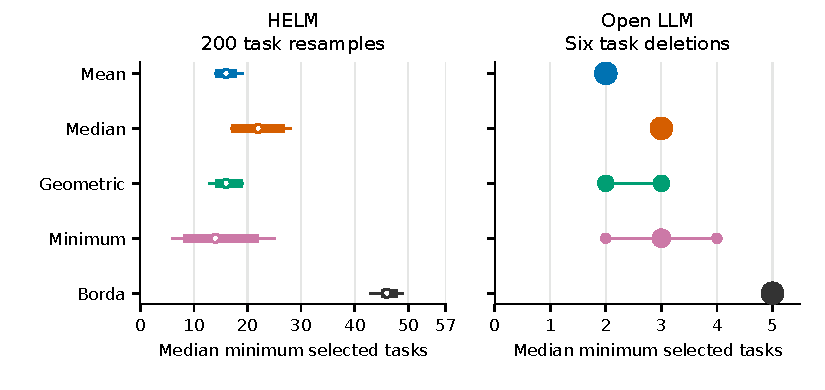
\includegraphics[width=\linewidth]{figures/task_composition.pdf}
\caption{\TaskCompositionCaption}
\label{fig:composition}
\end{figure}
\clearpage

\section{Reproduction and provenance}
\label{app:repro}
The delivery root contains the built \texttt{paper.pdf}, its source \texttt{paper.tex} and section sources under \texttt{manuscript/}. The exact dependencies and original environment are recorded in \texttt{reproduction/requirements.txt} and \texttt{reproduction/environment.json}. The analysis uses Python 3.11.2, NumPy 2.4.6, SciPy 1.17.1, pandas 3.0.6 and PyArrow 26.0.0. Runs use one BLAS/OpenMP thread and CPU only. Source acquisition time is separate from measured computation. The report sandbox allocation is two CPUs and 4,096 MB RAM; these are resource ceilings, not measured peak utilization or a claim about the analysis host's full hardware. Peak analysis memory was not recorded.

Run the acquisition and preparation scripts, then the validation and analysis commands in \texttt{reproduction/README.md}. Source versions, URLs and hashes are in \texttt{data/manifest.json}; acquisition checks retained hashes rather than silently accepting changed remote files. HELM downloads only release metadata and subject summaries, not a full mirror of model runs. Open LLM downloads one pinned parquet. The preparation audit records all exclusions and confirms complete finite matrices with scores in $[0,1]$.

\paragraph{Analysis files.}
\texttt{scripts/analysis.py} implements the intervention and exact optimizers, writes optimal subsets and solver metadata, and computes random-selection baselines. The full grid uses unit ceilings at $\alpha=1,0.5,0.25,0.1$ and observed maxima at $\alpha=1$. Its strict-first, raw-score and unique-model variants have separate output files. \texttt{scripts/robustness.py} generates task bootstrap and deletion results; \texttt{scripts/diagnostics.py} verifies winning subsets, monotonicity, uniqueness and unresolved statuses and produces random-baseline Monte Carlo intervals; \texttt{scripts/summarize.py} computes fixed-cohort summaries and paired counts. \texttt{tests/test\_solvers.py} compares optimizers with an independently enumerated reference. The seed for stochastic study outputs is 20261103; optimizer validation uses 47.

\paragraph{Numerical claim map.}
The primary common-challenger medians and paired exceptions are in \texttt{results/challenger\_summary.csv} and \texttt{results/challenger\_paired\_rules.csv}. Full-cohort medians, strict-first and raw/unique sensitivities are in \texttt{results/summary.csv}. Fixed-cohort reachability is in \texttt{results/budget\_curves.csv}; per-target selections and statuses are in \texttt{results/attacks\_*.csv}. The random-baseline cohort intervals are in \texttt{results/random\_baseline\_aggregate\_uncertainty.csv}; individual probabilities and Wilson intervals are in \texttt{results/random\_baseline\_uncertainty.csv}. Task-composition budgets and paired differences are in \texttt{results/composition\_*.csv} and \texttt{results/composition\_pairs\_*.csv}. Diagnostics are in \texttt{results/diagnostics.json}. Each rendered display is generated by \texttt{presentation/render.py}; its README maps all six table fragments and three figures to their caption macros, and its manifest records exact input and output hashes. The supplied numerical records identify models, task names, ceilings, gain fractions, solver status and selected subsets; no result depends on a manually chosen illustration.

\paragraph{Compute and failures.}
Measured full primary runs took 28.22 seconds for HELM and 71.41 seconds for Open LLM on the shared host. The 200 HELM bootstrap designs took 135.95 seconds; six Open LLM deletions took 23.39 seconds. Tracked analysis computation, including pilots and optimizer tests, used 316.972 CPU seconds. These are measurements on the recorded environment, not expected runtimes on all machines. All scheduled study computations completed. An initial optional acquisition-library import was unavailable; acquisition used Python's standard library without changing sources or methods. The delivered pilot timing outputs are excluded from study summaries. No model is trained, no model API is called, and no GPU is used.

\paragraph{Data rights and permitted literature.}
The public score sources do not separately declare a license for the score data. A code repository's Apache-2.0 license and individual model license metadata do not establish a license for the score tables; this delivery asserts none. The study uses public task-score summaries and does not collect personal data, model weights or question text. The task explicitly prohibited consulting an existing study of this particular question or material discussing it. We did not search for its identity or use it to frame novelty. The report position consulted the frozen instructions, supplied research evidence and the permitted sources recorded with the bibliography; no prohibited material was encountered by this position. Other source-access notes accompany the analysis and context records.

\section{Research assistance and reporting record}
\label{app:assistance}
LLM assistants contributed to research planning, permitted-source reading, algorithm implementation, analysis orchestration, figure generation, review and manuscript preparation. Their role extends beyond editing and formatting. The study's numerical observations are produced by the delivered deterministic or seeded programs operating on identified public score files; they are not language-model-generated measurements. Independent optimizer checks, direct reranking, hash verification and formal review provide checks on those programs and their exposition. LLM assistance does not establish scientific correctness; the delivered code, source evidence and reviewable numerical artifacts are the basis for assessing the claims.

The study plan was written after initial results were available and is explicitly evidence-informed, not a preregistration. All five declared rules, the full gain/ceiling grid, exceptions, infeasibility and completed robustness outputs are retained in the delivery. No human authors, affiliations, funding, model-training runs or institutional ethics approvals are invented for this report. The official NeurIPS 2026 style is used in public preprint mode, with no assertion of conference submission or acceptance.

\clearpage
\section*{NeurIPS Paper Checklist}




\begin{enumerate}

\item {\bf Claims}
    \item[] Question: Do the main claims made in the abstract and introduction accurately reflect the paper's contributions and scope?
    \item[] Answer: \answerYes{} % Replace by \answerYes{}, \answerNo{}, or \answerNA{}.
    \item[] Justification: The abstract and Sections~\ref{sec:methods}--\ref{sec:limitations} restrict all conclusions to the stated score-intervention menus and measured cohorts; no actual training efficacy or universal rule dominance is claimed.
    \item[] Guidelines:
    \begin{itemize}
        \item The answer \answerNA{} means that the abstract and introduction do not include the claims made in the paper.
        \item The abstract and/or introduction should clearly state the claims made, including the contributions made in the paper and important assumptions and limitations. A \answerNo{} or \answerNA{} answer to this question will not be perceived well by the reviewers. 
        \item The claims made should match theoretical and experimental results, and reflect how much the results can be expected to generalize to other settings. 
        \item It is fine to include aspirational goals as motivation as long as it is clear that these goals are not attained by the paper. 
    \end{itemize}

\item {\bf Limitations}
    \item[] Question: Does the paper discuss the limitations of the work performed by the authors?
    \item[] Answer: \answerYes{} % Replace by \answerYes{}, \answerNo{}, or \answerNA{}.
    \item[] Justification: Section~\ref{sec:limitations} discusses independent gains, unequal task costs, training attainability, fixed rivals, normalization, composition, noise and misuse.
    \item[] Guidelines:
    \begin{itemize}
        \item The answer \answerNA{} means that the paper has no limitation while the answer \answerNo{} means that the paper has limitations, but those are not discussed in the paper. 
        \item The authors are encouraged to create a separate ``Limitations'' section in their paper.
        \item The paper should point out any strong assumptions and how robust the results are to violations of these assumptions (e.g., independence assumptions, noiseless settings, model well-specification, asymptotic approximations only holding locally). The authors should reflect on how these assumptions might be violated in practice and what the implications would be.
        \item The authors should reflect on the scope of the claims made, e.g., if the approach was only tested on a few datasets or with a few runs. In general, empirical results often depend on implicit assumptions, which should be articulated.
        \item The authors should reflect on the factors that influence the performance of the approach. For example, a facial recognition algorithm may perform poorly when image resolution is low or images are taken in low lighting. Or a speech-to-text system might not be used reliably to provide closed captions for online lectures because it fails to handle technical jargon.
        \item The authors should discuss the computational efficiency of the proposed algorithms and how they scale with dataset size.
        \item If applicable, the authors should discuss possible limitations of their approach to address problems of privacy and fairness.
        \item While the authors might fear that complete honesty about limitations might be used by reviewers as grounds for rejection, a worse outcome might be that reviewers discover limitations that aren't acknowledged in the paper. The authors should use their best judgment and recognize that individual actions in favor of transparency play an important role in developing norms that preserve the integrity of the community. Reviewers will be specifically instructed to not penalize honesty concerning limitations.
    \end{itemize}

\item {\bf Theory assumptions and proofs}
    \item[] Question: For each theoretical result, does the paper provide the full set of assumptions and a complete (and correct) proof?
    \item[] Answer: \answerYes{} % Replace by \answerYes{}, \answerNo{}, or \answerNA{}.
    \item[] Justification: Section~\ref{sec:methods} states the assumptions and exact formulations; Appendix~\ref{app:proofs} supplies the complete exchange, threshold, pairwise and monotonicity arguments.
    \item[] Guidelines:
    \begin{itemize}
        \item The answer \answerNA{} means that the paper does not include theoretical results. 
        \item All the theorems, formulas, and proofs in the paper should be numbered and cross-referenced.
        \item All assumptions should be clearly stated or referenced in the statement of any theorems.
        \item The proofs can either appear in the main paper or the supplemental material, but if they appear in the supplemental material, the authors are encouraged to provide a short proof sketch to provide intuition. 
        \item Inversely, any informal proof provided in the core of the paper should be complemented by formal proofs provided in appendix or supplemental material.
        \item Theorems and Lemmas that the proof relies upon should be properly referenced. 
    \end{itemize}

    \item {\bf Experimental result reproducibility}
    \item[] Question: Does the paper fully disclose all the information needed to reproduce the main experimental results of the paper to the extent that it affects the main claims and/or conclusions of the paper (regardless of whether the code and data are provided or not)?
    \item[] Answer: \answerYes{} % Replace by \answerYes{}, \answerNo{}, or \answerNA{}.
    \item[] Justification: Section~\ref{sec:design} and Appendix~\ref{app:repro} disclose frozen matrices, construction, menus, tolerances, optimizers, checks, environments, seeds and commands, with the full code and numerical outputs attached.
    \item[] Guidelines:
    \begin{itemize}
        \item The answer \answerNA{} means that the paper does not include experiments.
        \item If the paper includes experiments, a \answerNo{} answer to this question will not be perceived well by the reviewers: Making the paper reproducible is important, regardless of whether the code and data are provided or not.
        \item If the contribution is a dataset and\slash or model, the authors should describe the steps taken to make their results reproducible or verifiable. 
        \item Depending on the contribution, reproducibility can be accomplished in various ways. For example, if the contribution is a novel architecture, describing the architecture fully might suffice, or if the contribution is a specific model and empirical evaluation, it may be necessary to either make it possible for others to replicate the model with the same dataset, or provide access to the model. In general. releasing code and data is often one good way to accomplish this, but reproducibility can also be provided via detailed instructions for how to replicate the results, access to a hosted model (e.g., in the case of a large language model), releasing of a model checkpoint, or other means that are appropriate to the research performed.
        \item While NeurIPS does not require releasing code, the conference does require all submissions to provide some reasonable avenue for reproducibility, which may depend on the nature of the contribution. For example
        \begin{enumerate}
            \item If the contribution is primarily a new algorithm, the paper should make it clear how to reproduce that algorithm.
            \item If the contribution is primarily a new model architecture, the paper should describe the architecture clearly and fully.
            \item If the contribution is a new model (e.g., a large language model), then there should either be a way to access this model for reproducing the results or a way to reproduce the model (e.g., with an open-source dataset or instructions for how to construct the dataset).
            \item We recognize that reproducibility may be tricky in some cases, in which case authors are welcome to describe the particular way they provide for reproducibility. In the case of closed-source models, it may be that access to the model is limited in some way (e.g., to registered users), but it should be possible for other researchers to have some path to reproducing or verifying the results.
        \end{enumerate}
    \end{itemize}


\item {\bf Open access to data and code}
    \item[] Question: Does the paper provide open access to the data and code, with sufficient instructions to faithfully reproduce the main experimental results, as described in supplemental material?
    \item[] Answer: \answerYes{} % Replace by \answerYes{}, \answerNo{}, or \answerNA{}.
    \item[] Justification: Appendix~\ref{app:repro} and the attached reproduction instructions provide code, prepared matrices, numerical outputs and hash-verified acquisition from public unauthenticated sources; upstream score-data licensing remains unknown as disclosed in item 12.
    \item[] Guidelines:
    \begin{itemize}
        \item The answer \answerNA{} means that paper does not include experiments requiring code.
        \item Please see the NeurIPS code and data submission guidelines (\url{https://neurips.cc/public/guides/CodeSubmissionPolicy}) for more details.
        \item While we encourage the release of code and data, we understand that this might not be possible, so \answerNo{} is an acceptable answer. Papers cannot be rejected simply for not including code, unless this is central to the contribution (e.g., for a new open-source benchmark).
        \item The instructions should contain the exact command and environment needed to run to reproduce the results. See the NeurIPS code and data submission guidelines (\url{https://neurips.cc/public/guides/CodeSubmissionPolicy}) for more details.
        \item The authors should provide instructions on data access and preparation, including how to access the raw data, preprocessed data, intermediate data, and generated data, etc.
        \item The authors should provide scripts to reproduce all experimental results for the new proposed method and baselines. If only a subset of experiments are reproducible, they should state which ones are omitted from the script and why.
        \item At submission time, to preserve anonymity, the authors should release anonymized versions (if applicable).
        \item Providing as much information as possible in supplemental material (appended to the paper) is recommended, but including URLs to data and code is permitted.
    \end{itemize}


\item {\bf Experimental setting/details}
    \item[] Question: Does the paper specify all the training and test details (e.g., data splits, hyperparameters, how they were chosen, type of optimizer) necessary to understand the results?
    \item[] Answer: \answerYes{} % Replace by \answerYes{}, \answerNo{}, or \answerNA{}.
    \item[] Justification: Sections~\ref{sec:methods} and \ref{sec:design} define every score-processing and optimization setting. No model is trained or newly evaluated; no unreported training hyperparameters are involved.
    \item[] Guidelines:
    \begin{itemize}
        \item The answer \answerNA{} means that the paper does not include experiments.
        \item The experimental setting should be presented in the core of the paper to a level of detail that is necessary to appreciate the results and make sense of them.
        \item The full details can be provided either with the code, in appendix, or as supplemental material.
    \end{itemize}

\item {\bf Experiment statistical significance}
    \item[] Question: Does the paper report error bars suitably and correctly defined or other appropriate information about the statistical significance of the experiments?
    \item[] Answer: \answerYes{} % Replace by \answerYes{}, \answerNo{}, or \answerNA{}.
    \item[] Justification: Sections~\ref{sec:design} and \ref{sec:results} separate exact finite-cohort budgets from random-task-order Monte Carlo intervals and task-composition sensitivity ranges; the absence of identifiable score uncertainty is explicit.
    \item[] Guidelines:
    \begin{itemize}
        \item The answer \answerNA{} means that the paper does not include experiments.
        \item The authors should answer \answerYes{} if the results are accompanied by error bars, confidence intervals, or statistical significance tests, at least for the experiments that support the main claims of the paper.
        \item The factors of variability that the error bars are capturing should be clearly stated (for example, train/test split, initialization, random drawing of some parameter, or overall run with given experimental conditions).
        \item The method for calculating the error bars should be explained (closed form formula, call to a library function, bootstrap, etc.)
        \item The assumptions made should be given (e.g., Normally distributed errors).
        \item It should be clear whether the error bar is the standard deviation or the standard error of the mean.
        \item It is OK to report 1-sigma error bars, but one should state it. The authors should preferably report a 2-sigma error bar than state that they have a 96\% CI, if the hypothesis of Normality of errors is not verified.
        \item For asymmetric distributions, the authors should be careful not to show in tables or figures symmetric error bars that would yield results that are out of range (e.g., negative error rates).
        \item If error bars are reported in tables or plots, the authors should explain in the text how they were calculated and reference the corresponding figures or tables in the text.
    \end{itemize}

\item {\bf Experiments compute resources}
    \item[] Question: For each experiment, does the paper provide sufficient information on the computer resources (type of compute workers, memory, time of execution) needed to reproduce the experiments?
    \item[] Answer: \answerYes{} % Replace by \answerYes{}, \answerNo{}, or \answerNA{}.
    \item[] Justification: Appendix~\ref{app:repro} and the reproduction environment/run records give CPU-only computation, measured run times, threading and total tracked analysis compute including pilots and tests; the documented resource limits are distinguished from measured usage.
    \item[] Guidelines:
    \begin{itemize}
        \item The answer \answerNA{} means that the paper does not include experiments.
        \item The paper should indicate the type of compute workers CPU or GPU, internal cluster, or cloud provider, including relevant memory and storage.
        \item The paper should provide the amount of compute required for each of the individual experimental runs as well as estimate the total compute. 
        \item The paper should disclose whether the full research project required more compute than the experiments reported in the paper (e.g., preliminary or failed experiments that didn't make it into the paper). 
    \end{itemize}
    
\item {\bf Code of ethics}
    \item[] Question: Does the research conducted in the paper conform, in every respect, with the NeurIPS Code of Ethics \url{https://neurips.cc/public/EthicsGuidelines}?
    \item[] Answer: \answerYes{} % Replace by \answerYes{}, \answerNo{}, or \answerNA{}.
    \item[] Justification: We read the NeurIPS Code of Ethics at its official URL on 2026-11-03. This is a public-score audit without human participants or model deployment; Section~\ref{sec:limitations} addresses representation and misuse, and Appendix~\ref{app:repro} discloses unknown asset licenses rather than assuming permission.
    \item[] Guidelines:
    \begin{itemize}
        \item The answer \answerNA{} means that the authors have not reviewed the NeurIPS Code of Ethics.
        \item If the authors answer \answerNo, they should explain the special circumstances that require a deviation from the Code of Ethics.
        \item The authors should make sure to preserve anonymity (e.g., if there is a special consideration due to laws or regulations in their jurisdiction).
    \end{itemize}


\item {\bf Broader impacts}
    \item[] Question: Does the paper discuss both potential positive societal impacts and negative societal impacts of the work performed?
    \item[] Answer: \answerYes{} % Replace by \answerYes{}, \answerNo{}, or \answerNA{}.
    \item[] Justification: Section~\ref{sec:limitations} discusses defensive benchmark design and the possibility that released optimization tools reveal gaming opportunities; no model or contamination intervention is deployed.
    \item[] Guidelines:
    \begin{itemize}
        \item The answer \answerNA{} means that there is no societal impact of the work performed.
        \item If the authors answer \answerNA{} or \answerNo, they should explain why their work has no societal impact or why the paper does not address societal impact.
        \item Examples of negative societal impacts include potential malicious or unintended uses (e.g., disinformation, generating fake profiles, surveillance), fairness considerations (e.g., deployment of technologies that could make decisions that unfairly impact specific groups), privacy considerations, and security considerations.
        \item The conference expects that many papers will be foundational research and not tied to particular applications, let alone deployments. However, if there is a direct path to any negative applications, the authors should point it out. For example, it is legitimate to point out that an improvement in the quality of generative models could be used to generate Deepfakes for disinformation. On the other hand, it is not needed to point out that a generic algorithm for optimizing neural networks could enable people to train models that generate Deepfakes faster.
        \item The authors should consider possible harms that could arise when the technology is being used as intended and functioning correctly, harms that could arise when the technology is being used as intended but gives incorrect results, and harms following from (intentional or unintentional) misuse of the technology.
        \item If there are negative societal impacts, the authors could also discuss possible mitigation strategies (e.g., gated release of models, providing defenses in addition to attacks, mechanisms for monitoring misuse, mechanisms to monitor how a system learns from feedback over time, improving the efficiency and accessibility of ML).
    \end{itemize}
    
\item {\bf Safeguards}
    \item[] Question: Does the paper describe safeguards that have been put in place for responsible release of data or models that have a high risk for misuse (e.g., pre-trained language models, image generators, or scraped datasets)?
    \item[] Answer: \answerNA{} % Replace by \answerYes{}, \answerNo{}, or \answerNA{}.
    \item[] Justification: The released artifacts are public-score analysis code and derived numerical results, with no pretrained model, unsafe content corpus or personal-data collection. The direct incentive/misuse concern is disclosed in Section~\ref{sec:limitations}.
    \item[] Guidelines:
    \begin{itemize}
        \item The answer \answerNA{} means that the paper poses no such risks.
        \item Released models that have a high risk for misuse or dual-use should be released with necessary safeguards to allow for controlled use of the model, for example by requiring that users adhere to usage guidelines or restrictions to access the model or implementing safety filters. 
        \item Datasets that have been scraped from the Internet could pose safety risks. The authors should describe how they avoided releasing unsafe images.
        \item We recognize that providing effective safeguards is challenging, and many papers do not require this, but we encourage authors to take this into account and make a best faith effort.
    \end{itemize}

\item {\bf Licenses for existing assets}
    \item[] Question: Are the creators or original owners of assets (e.g., code, data, models), used in the paper, properly credited and are the license and terms of use explicitly mentioned and properly respected?
    \item[] Answer: \answerNo{} % Replace by \answerYes{}, \answerNo{}, or \answerNA{}.
    \item[] Justification: The original benchmark and leaderboard creators are credited and exact versions/URLs are recorded, but no separate score-data license was found. Appendix~\ref{app:repro} and the source manifest disclose this uncertainty; model/code licenses are not represented as score-data licenses.
    \item[] Guidelines:
    \begin{itemize}
        \item The answer \answerNA{} means that the paper does not use existing assets.
        \item The authors should cite the original paper that produced the code package or dataset.
        \item The authors should state which version of the asset is used and, if possible, include a URL.
        \item The name of the license (e.g., CC-BY 4.0) should be included for each asset.
        \item For scraped data from a particular source (e.g., website), the copyright and terms of service of that source should be provided.
        \item If assets are released, the license, copyright information, and terms of use in the package should be provided. For popular datasets, \url{paperswithcode.com/datasets} has curated licenses for some datasets. Their licensing guide can help determine the license of a dataset.
        \item For existing datasets that are re-packaged, both the original license and the license of the derived asset (if it has changed) should be provided.
        \item If this information is not available online, the authors are encouraged to reach out to the asset's creators.
    \end{itemize}

\item {\bf New assets}
    \item[] Question: Are new assets introduced in the paper well documented and is the documentation provided alongside the assets?
    \item[] Answer: \answerYes{} % Replace by \answerYes{}, \answerNo{}, or \answerNA{}.
    \item[] Justification: Appendix~\ref{app:repro}, root README and reproduction/presentation manifests document the new analysis code, exact outputs, environments, seeds, provenance, generators and interpretation limits alongside the delivered artifacts.
    \item[] Guidelines:
    \begin{itemize}
        \item The answer \answerNA{} means that the paper does not release new assets.
        \item Researchers should communicate the details of the dataset\slash code\slash model as part of their submissions via structured templates. This includes details about training, license, limitations, etc. 
        \item The paper should discuss whether and how consent was obtained from people whose asset is used.
        \item At submission time, remember to anonymize your assets (if applicable). You can either create an anonymized URL or include an anonymized zip file.
    \end{itemize}

\item {\bf Crowdsourcing and research with human subjects}
    \item[] Question: For crowdsourcing experiments and research with human subjects, does the paper include the full text of instructions given to participants and screenshots, if applicable, as well as details about compensation (if any)? 
    \item[] Answer: \answerNA{} % Replace by \answerYes{}, \answerNo{}, or \answerNA{}.
    \item[] Justification: This study uses public aggregate model-evaluation score tables and involves no crowdsourcing or human-subject experiments.
    \item[] Guidelines:
    \begin{itemize}
        \item The answer \answerNA{} means that the paper does not involve crowdsourcing nor research with human subjects.
        \item Including this information in the supplemental material is fine, but if the main contribution of the paper involves human subjects, then as much detail as possible should be included in the main paper. 
        \item According to the NeurIPS Code of Ethics, workers involved in data collection, curation, or other labor should be paid at least the minimum wage in the country of the data collector. 
    \end{itemize}

\item {\bf Institutional review board (IRB) approvals or equivalent for research with human subjects}
    \item[] Question: Does the paper describe potential risks incurred by study participants, whether such risks were disclosed to the subjects, and whether Institutional Review Board (IRB) approvals (or an equivalent approval/review based on the requirements of your country or institution) were obtained?
    \item[] Answer: \answerNA{} % Replace by \answerYes{}, \answerNo{}, or \answerNA{}.
    \item[] Justification: There are no recruited participants or human-subject experiments, and no IRB approval is claimed.
    \item[] Guidelines:
    \begin{itemize}
        \item The answer \answerNA{} means that the paper does not involve crowdsourcing nor research with human subjects.
        \item Depending on the country in which research is conducted, IRB approval (or equivalent) may be required for any human subjects research. If you obtained IRB approval, you should clearly state this in the paper. 
        \item We recognize that the procedures for this may vary significantly between institutions and locations, and we expect authors to adhere to the NeurIPS Code of Ethics and the guidelines for their institution. 
        \item For initial submissions, do not include any information that would break anonymity (if applicable), such as the institution conducting the review.
    \end{itemize}

\item {\bf Declaration of LLM usage}
    \item[] Question: Does the paper describe the usage of LLMs if it is an important, original, or non-standard component of the core methods in this research? Note that if the LLM is used only for writing, editing, or formatting purposes and does \emph{not} impact the core methodology, scientific rigor, or originality of the research, declaration is not required.
    %this research? 
    \item[] Answer: \answerYes{} % Replace by \answerYes{}, \answerNo{}, or \answerNA{}.
    \item[] Justification: Appendix~\ref{app:assistance} discloses that LLM assistants contributed to study design, implementation, source reading, analysis and manuscript preparation, beyond writing alone. Numerical findings come from executable calculations and independent checks, not generated observations.
    \item[] Guidelines:
    \begin{itemize}
        \item The answer \answerNA{} means that the core method development in this research does not involve LLMs as any important, original, or non-standard components.
        \item Please refer to our LLM policy in the NeurIPS handbook for what should or should not be described.
    \end{itemize}

\end{enumerate}
\end{document}
